% $Id: INF_Poster_example.tex 7714 2011-08-31 17:34:46Z tkren $
%
% TU Wien - Faculty of Informatics
% poster template
%
% This template is using the beamer document class and beamerposter package, see
% <http://www.ctan.org/tex-archive/macros/latex/contrib/beamer/>
% <http://www.ctan.org/tex-archive/macros/latex/contrib/beamerposter/>
% <http://www-i6.informatik.rwth-aachen.de/~dreuw/latexbeamerposter.php>
%
% For questions and comments send an email to
% Thomas Krennwallner <tkren@kr.tuwien.ac.at>
%

\documentclass[final,hyperref={pdfpagelabels=true}]{beamer}

\usepackage{minted}
%\usepackage{ucs}
\usepackage{TUINFPST}
\usepackage{listings}
\usepackage{wrapfig}
\usepackage{comment}

\usepackage[scaled]{beramono}
\fvset{fontsize=\tiny}

\usemintedstyle{perldoc}

%\usepackage{ucs}

%\title[Computational Intelligence]{Interactive Computer Generated Architecture}
% if you have a long title looking squeezed on the poster, just force
% some distance:
\title[Software Engineering \& Internet Computing]{%
  A Weather Ontology for \\[0.2\baselineskip]%
  Predictive Control in Smart Homes %\\[0.2\baselineskip]%
}
\author[paulchen@rueckgr.at]{Paul Staroch}
\institute[]{%
  Technische Universit{\"a}t Wien\\[0.25\baselineskip]
  Institut für Rechnergestützte Automation\\[0.25\baselineskip]
  Arbeitsbereich: Automatisierungssysteme\\[0.25\baselineskip]
  Betreuung: Ao.Univ.-Prof. Dipl.-Ing. Dr.techn. Wolfgang Kastner\\[0.25\baselineskip]
  Mitwirkung: Dipl.-Ing. Mario Kofler
}
\titlegraphic{
\includegraphics[height=52mm]{figures/183-1.pdf}}
\date[\today]{\today}
\subject{epilog}
\keywords{Gebäudeautomation, Smart Homes, Ontologien} % TODO

%%%%%%%%%%%%%%%%%%%%%%%%%%%%%%%%%%%%%%%%%%%%%%%%%%%%%%%%%%%%%%%%%%%%%%%%%%%%%%%%%%%%%%

% Display a grid to help align images 
%\beamertemplategridbackground[12.7mm]

% play around with the background colors
%\setbeamercolor{background canvas}{bg=yellow}

% use a background picture
\usebackgroundtemplate{%
  \ifdefined\isprint
    \includegraphics[width=\paperwidth,height=\paperheight]{figures/background_cmyk.jpg}
  \else
    \includegraphics[width=\paperwidth,height=\paperheight]{figures/background.jpg}
  \fi

}

% play around with block colors
\setbeamercolor{block body}{fg=black,bg=white}
\setbeamercolor{block title}{fg=TuWienBlue,bg=white}

\definecolor{TuWienBlueLight}{cmyk}{.1,.1,.1,.3}
\definecolor{listingBottom}{cmyk}{.1,.1,.1,.1}

\setbeamertemplate{block begin}{
  \pgfsetfillopacity{0.7}
  \begin{beamercolorbox}{block title}%
    \begin{tikzpicture}%
      \node[draw,rectangle,line width=3pt,rounded corners=0pt,inner sep=0pt,shade,top color=white,bottom color=TuWienBlueLight]{%
        \begin{minipage}[c][2cm]{\linewidth}
          \centering\textbf{\insertblocktitle}
        \end{minipage}
      };
    \end{tikzpicture}%
  \end{beamercolorbox}
  \begin{beamercolorbox}[colsep=1.5pt,sep=1cm]{block body}%
%  \vspace*{.5cm}
}

\setbeamertemplate{block end}{
  \end{beamercolorbox}
  \vspace{1cm}
}

% setup postit
%\setbeamercolor{postit}{fg=black,bg=yellow} 
%\newenvironment{postit}
%{\begin{beamercolorbox}[sep=1em,wd=7cm]{postit}}
%{\end{beamercolorbox}}


% for crop marks, uncomment the following line
\ifdefined\isprint
  \usepackage[cross,width=88truecm,height=123truecm,center]{crop}
\fi

%%%%%%%%%%%%%%%%%%%%%%%%%%%%%%%%%%%%%%%%%%%%%%%%%%%%%%%%%%%%%%%%%%%%%%%%%%%%%%%%%%%%%%

%\lstset{frame=trbl,basicstyle=\scriptsize,moredelim=**[is][{\btHL[fill=green!20]}]{@@}{@@},}
%\lstset{frame=trBL,basicstyle=\normalsize}

% \setlength{\parskip}{15em}

% \addtobeamertemplate{block begin}{\pgfsetfillopacity{0.5}}{\pgfsetfillopacity{1}}

\DeclareUnicodeCharacter{21D2}{$\Rightarrow$}
\DeclareUnicodeCharacter{2227}{$\wedge$}
%\DeclareUnicodeCharacter{00A0}{~}

%\PrerenderUnicode{⇒}
%\PrerenderUnicode{∧}

\begin{document}

% We have a single poster frame.
\begin{frame}[fragile]
  \begin{columns}[t]
    % ---------------------------------------------------------%
    % Set up a column
    \begin{column}{.45\textwidth}
      \begin{block}{Smart homes and ontologies}
        \begin{wrapfigure}{r}{.45\textwidth}
	  \centering
	  \vspace{-1em}
	  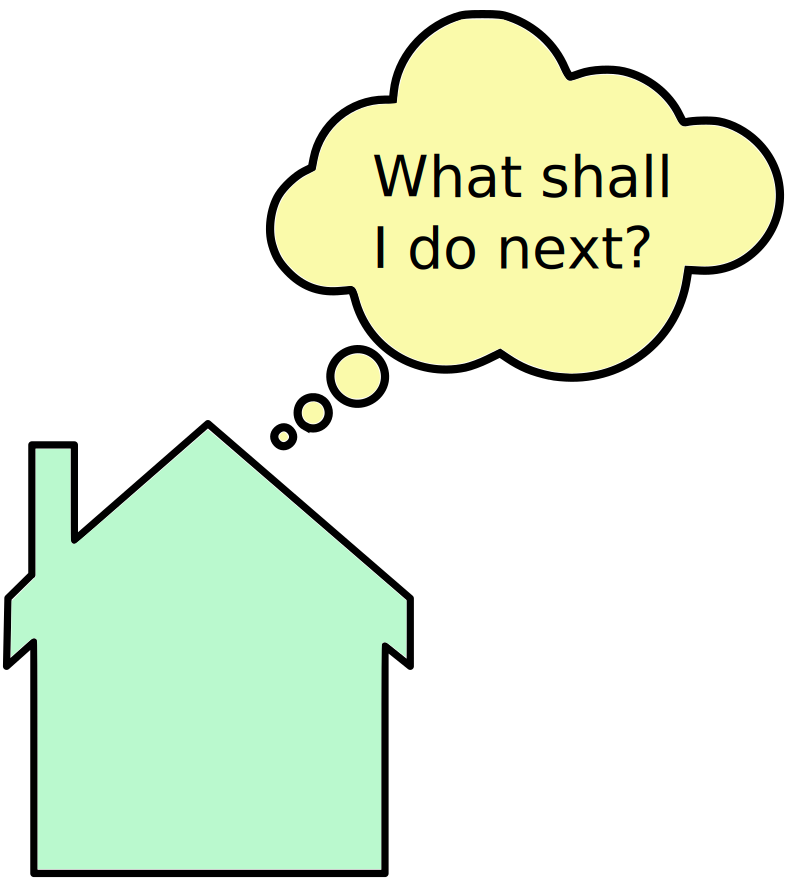
\includegraphics[width=.31\textwidth]{figures/inkscape/smart_home}
	\end{wrapfigure}

	\vspace{-1.5em}
	
	\emph{Smart homes} are dwellings that are equipped\\
	\mbox{with some kind of intelligence to perform}
	tasks on their own.

	\vspace{.5em}
	Some of their goals are:

	\begin{itemize}
	  \item \mbox{Support with routine tasks.}
	  \item Increase comfort.
	  \item \mbox{Reduce energy consumption.}
        \end{itemize}

	\vspace{.5em}
	\mbox{Common problems of many smart home systems:}

        \begin{itemize}
	  \item High complexity.
	  \item Optimising and customising are difficult.
	  \item Missing powerfulness and flexibility.
	\end{itemize}

	\vspace{.5em}
	To overcome these problems, a knowledge
	base built upon \emph{OWL} can be introduced.
	A smart home can use the knowledge from this
	model to make appropriate control decisions.
      \end{block}

      \begin{block}{Why introduce a weather data model?}
        \begin{wrapfigure}{r}{.55\textwidth}
	  \vspace{-.5em}
	  \centering
	  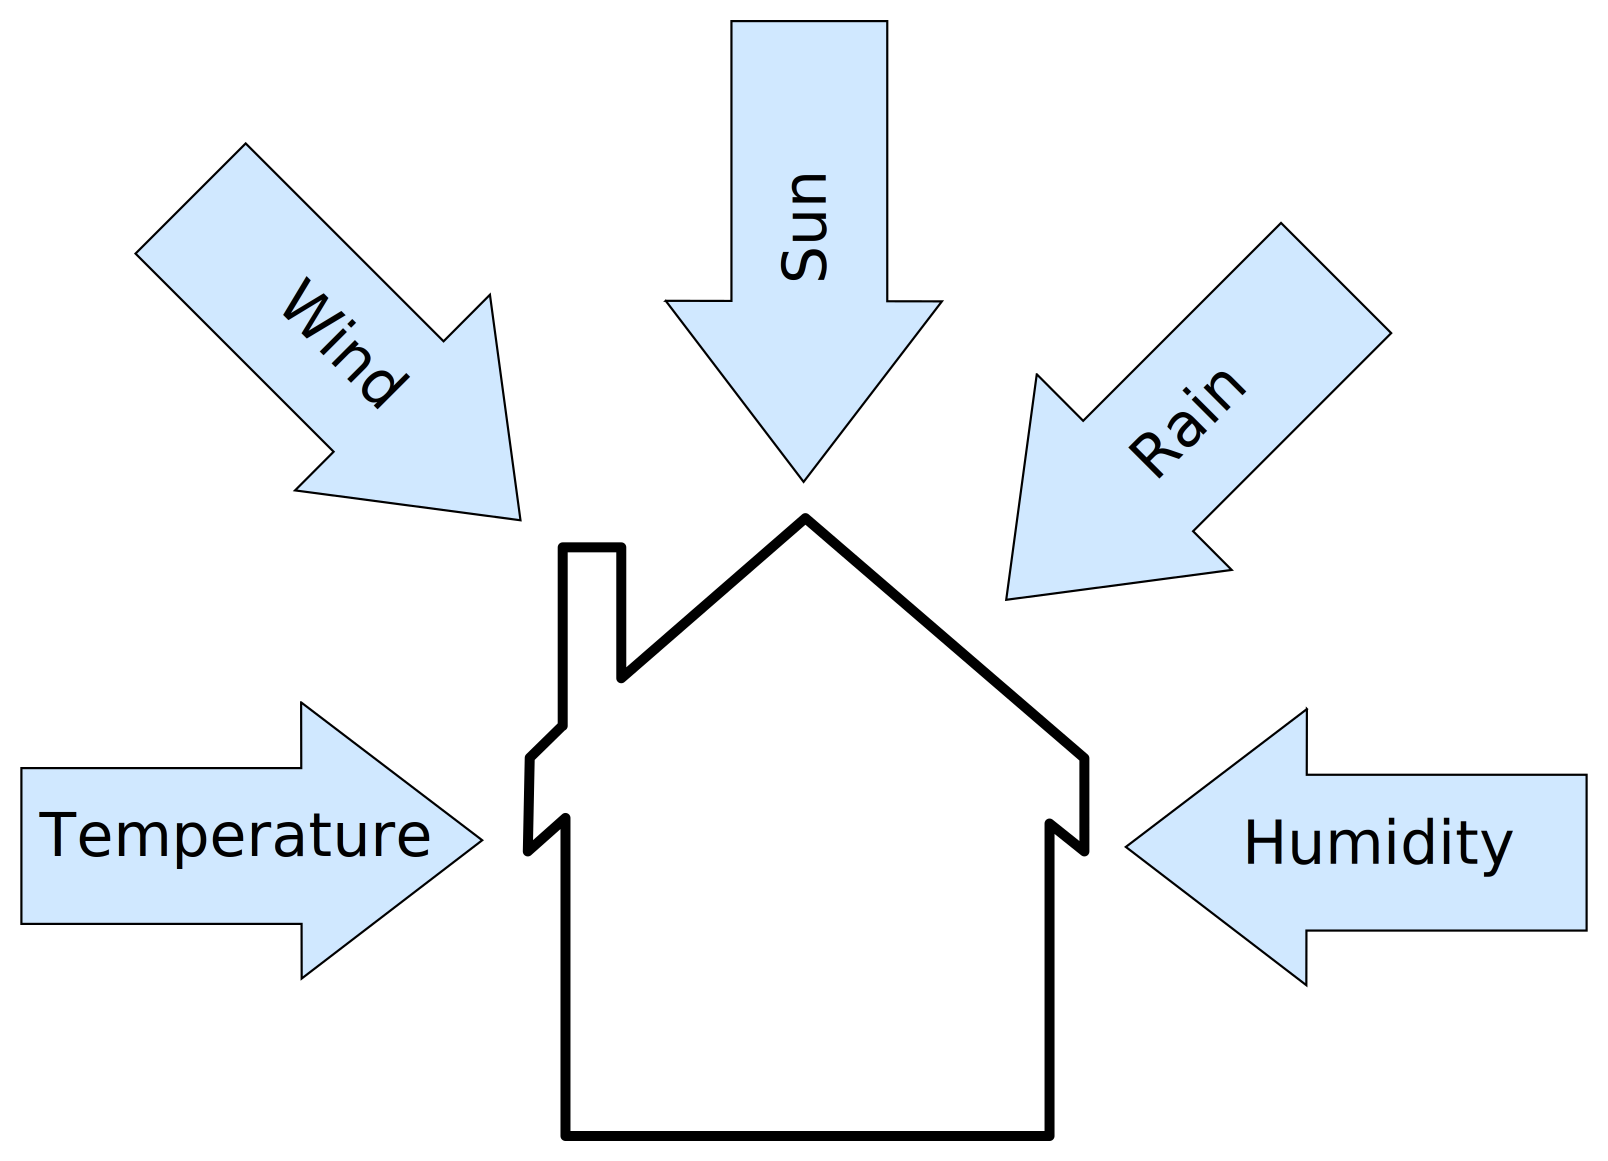
\includegraphics[width=.45\textwidth]{figures/inkscape/house}
	\end{wrapfigure}

	\vspace{-1.5em}
	
	\mbox{Weather has a wide influence on}
	\mbox{a dwelling. Examples for weather-}
	\mbox{related control decisions are:}
	
	\begin{itemize}
  	  \item Heating, ventilation, and air conditioning (\emph{HVAC}).
	  \item Irrigation.
	  \item \mbox{Utilisation of solar and} wind power.
	\end{itemize}

	\vspace{-.2em}
	\begin{itemize}
	  \item Preparing for severe weather (e.g.\ close windows, retract awnings).
	\end{itemize}
      \end{block}

      \begin{block}{Methodological approach}
	\vspace{-.5em}
	\begin{itemize}
	  \item Evaluation of existing weather ontologies.
	  \item Identification of uses cases for weather data in smart homes.
	  \item Analysis of methodologies for ontology design.
	  \item Examination of sources for weather data.
	  \item Design of \emph{SmartHomeWeather} using \emph{METHONTOLOGY}. % ~\cite{Methontology}.
	  \item Development of \emph{Weather Importer}.
	\end{itemize}
      \end{block}

      \begin{block}{The \emph{SmartHomeWeather} ontology}
        \begin{wrapfigure}{r}{.55\textwidth}
	  \vspace{-.5em}
	  \centering
  	  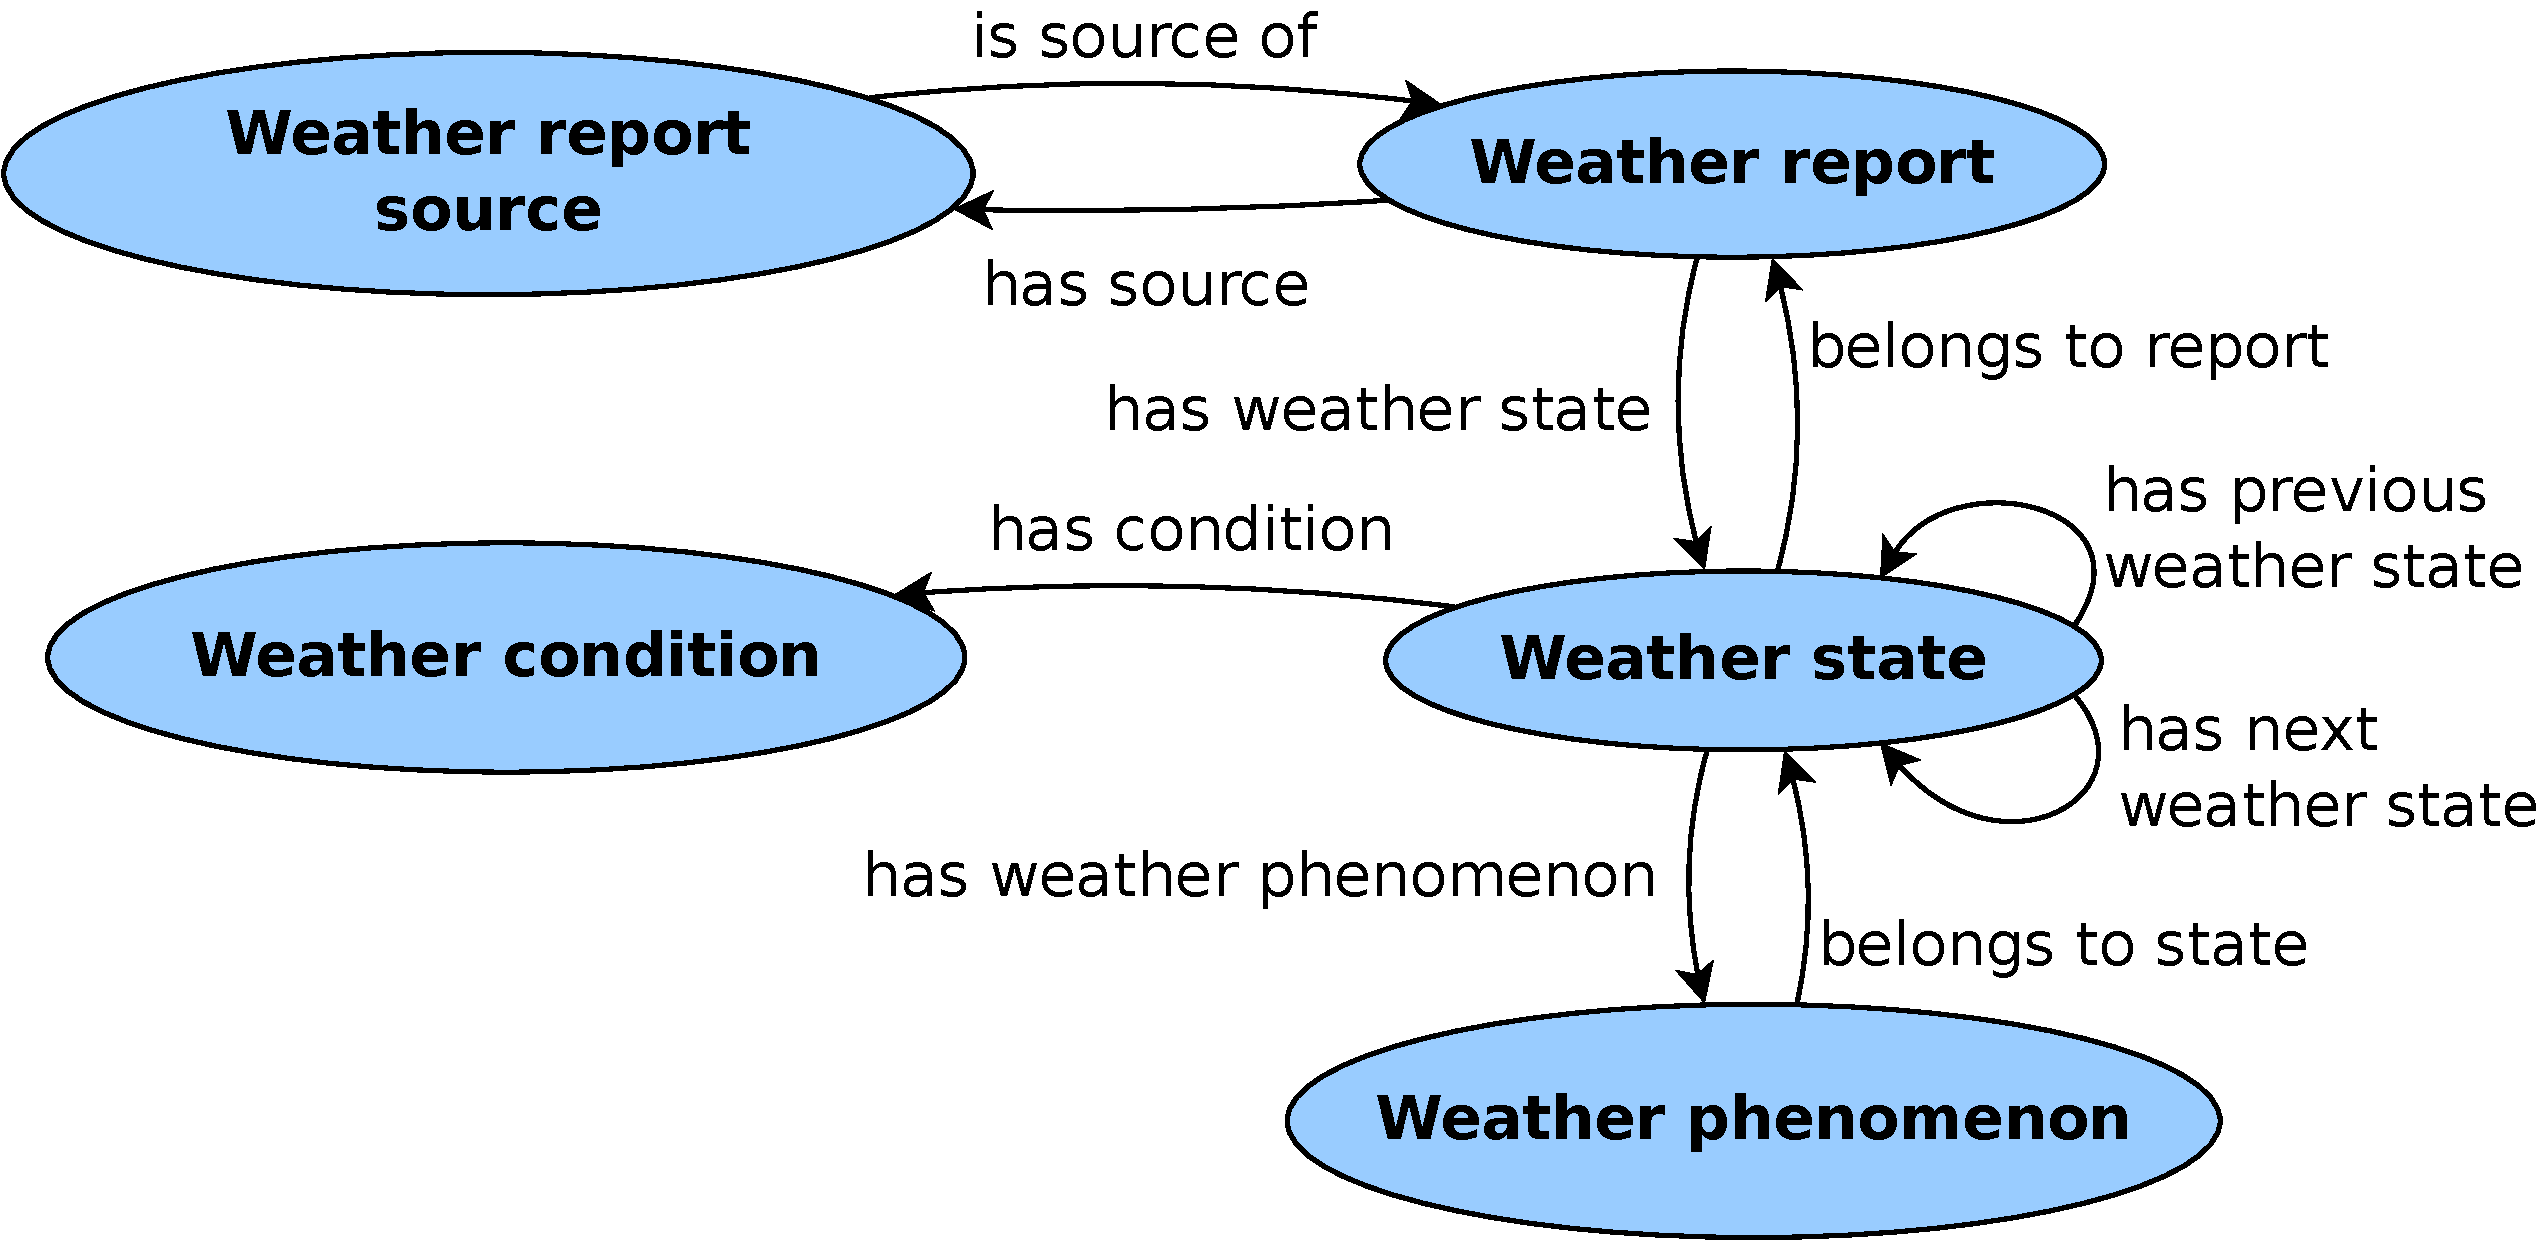
\includegraphics[width=.45\textwidth]{figures/dia/binary-relations}
	\end{wrapfigure}

	\vspace{-1.5em}

	\begin{itemize}
	  \item The \emph{SmartHomeWeather} ontology is built around five top-level concepts.
	  \item It supports current and future weather data.
	  \item It allows weather-based control decisions within smart home systems.
	  \item \emph{SmartHomeWeather} \mbox{uses \emph{OWL} reasoning} heavily.
	\end{itemize}

	\vspace{1.5em}
      \end{block}
    \end{column}
    % ---------------------------------------------------------%
    % end the column

    % ---------------------------------------------------------%
    % Set up a column 
    \begin{column}{.45\textwidth}
      \begin{block}{The \emph{SmartHomeWeather} ontology (cont.)}
	\vspace{-.25em}

	The top-level concepts are:

	\begin{itemize}
  	  \item \emph{Weather phenomenon}: A certain weather
		  element: temperature, humidity, …
	  \item \emph{Weather condition}: A one-word description of the
		  weather situation: ``Sun'', ``Fog'', …
	  \item \emph{Weather state}: The weather situation as a
		  set of \emph{Weather} \emph{phenomena}.
	  \item \emph{Weather report}: All data about the weather for one
		  point of time (location, source, weather situation).
	\end{itemize}
	\hspace{-1.05cm}\begin{minipage}{\dimexpr.45\textwidth}
	  \vspace{.3em}
	  \begin{itemize}
  	    \item \emph{Weather report source}: \mbox{A source of weather data}
	  	  (sensor or Internet service)
	  \end{itemize}

	  \vspace{.5em}

	  \hfill\begin{minipage}{\dimexpr\textwidth-1.05cm}
	  \raggedright
	  Each concept is root \mbox{of a concept hierarchy.}
	  \end{minipage}
	\end{minipage}
	\begin{minipage}{\dimexpr.5\textwidth}
	  \centering
	  \vspace{2em}
  	  \includegraphics[width=\textwidth]{figures/dia/hierarchy}
	\end{minipage}

	\vspace{2em}

	Querying the data model is done using \emph{SWRL} rules and \emph{SPARQL} queries.

	\vspace{10mm}
	\begin{minipage}[t]{.5\textwidth}
	\raggedright
	\begin{tikzpicture}%
          \node[draw,rectangle,line width=3pt,rounded corners=0pt,inner sep=0pt,shade,top color=white,bottom color=listingBottom]{%
	    \begin{minipage}{\dimexpr\textwidth-2cm}
	      \hspace{5mm}
              \begin{minipage}{\dimexpr\textwidth-2cm}
              \vspace{11mm}
	      \ttfamily\tiny
\noindent hasWeatherPhenomenon(?s1, ?t1) $\wedge$

~~hasTemperatureValue(?t1, ?v1) $\wedge$

\vspace{1.5em}
~~hasWeatherPhenomenon(?s2, ?t2) $\wedge$

~~hasTemperatureValue(?t2, ?v2) $\wedge$

\vspace{1.45em}
~~greaterThan(?v2, ?v1) $\wedge$

~~hasNextWeatherState(?s1, ?s2) $\Rightarrow$

~~~~increasingTemperature(?s1, ?s2)
    	      \vspace{10mm}
	      \end{minipage}
            \end{minipage}
	  };
	\end{tikzpicture}
	\begin{minipage}[t]{.87\textwidth}
	  \vspace{-1em}\raggedright\scriptsize\emph{SWRL} rule (simplified) to find consecutive \emph{Weather state}s that denote increasing temperature.
        \end{minipage}
	\end{minipage}\begin{minipage}[t]{.5\textwidth}
	\raggedright
	\begin{tikzpicture}%
          \node[draw,rectangle,line width=3pt,rounded corners=0pt,inner sep=0pt,shade,top color=white,bottom color=listingBottom]{%
	    \begin{minipage}{\dimexpr\textwidth-2cm}
	      \hspace{5mm}
              \begin{minipage}{\dimexpr\textwidth-2cm}
              \vspace{10mm}
% WHERE {
    	      \begin{minted}{sparql}
SELECT ?s2
WHERE {
    ?s1 weather:increasingTemperature ?s2.
    ?s1 weather:belongsToWeatherReport ?r.
    ?r a weather:ShortRangeForecastReport.
}
  
 
 
 
 
    	      \end{minted}
    	      \vspace{33.4mm}
	      \end{minipage}
            \end{minipage}
	  };
	\end{tikzpicture}
	\begin{minipage}[t]{.87\textwidth}
	  \vspace{-1em}\raggedright\scriptsize\emph{SPARQL} query to obtain all \emph{Weather states} for the upcoming three hours (\texttt{ShortRangeForecast- Report}) that denote increasing temperature (refer to the \emph{SWRL} rule seen on the left).

~
        \end{minipage}
	\end{minipage}	
      \end{block}
      
      \begin{block}{The \emph{Weather Importer}}
        \begin{minipage}{\dimexpr.49\textwidth}
	  \mbox{The \emph{Weather Importer}}

	  \hspace{-.84em}\begin{minipage}{\dimexpr\textwidth+.84em}
	    \vspace{.4em}
	    \begin{itemize}
	      \item is implemented in Java.
	      \item \mbox{uses an object-oriented model} resembling the structure of \emph{SmartHomeWeather}.
	    \end{itemize}
	  \end{minipage}
	\end{minipage}
	\begin{minipage}{\dimexpr.41\textwidth}
	  \centering
  	  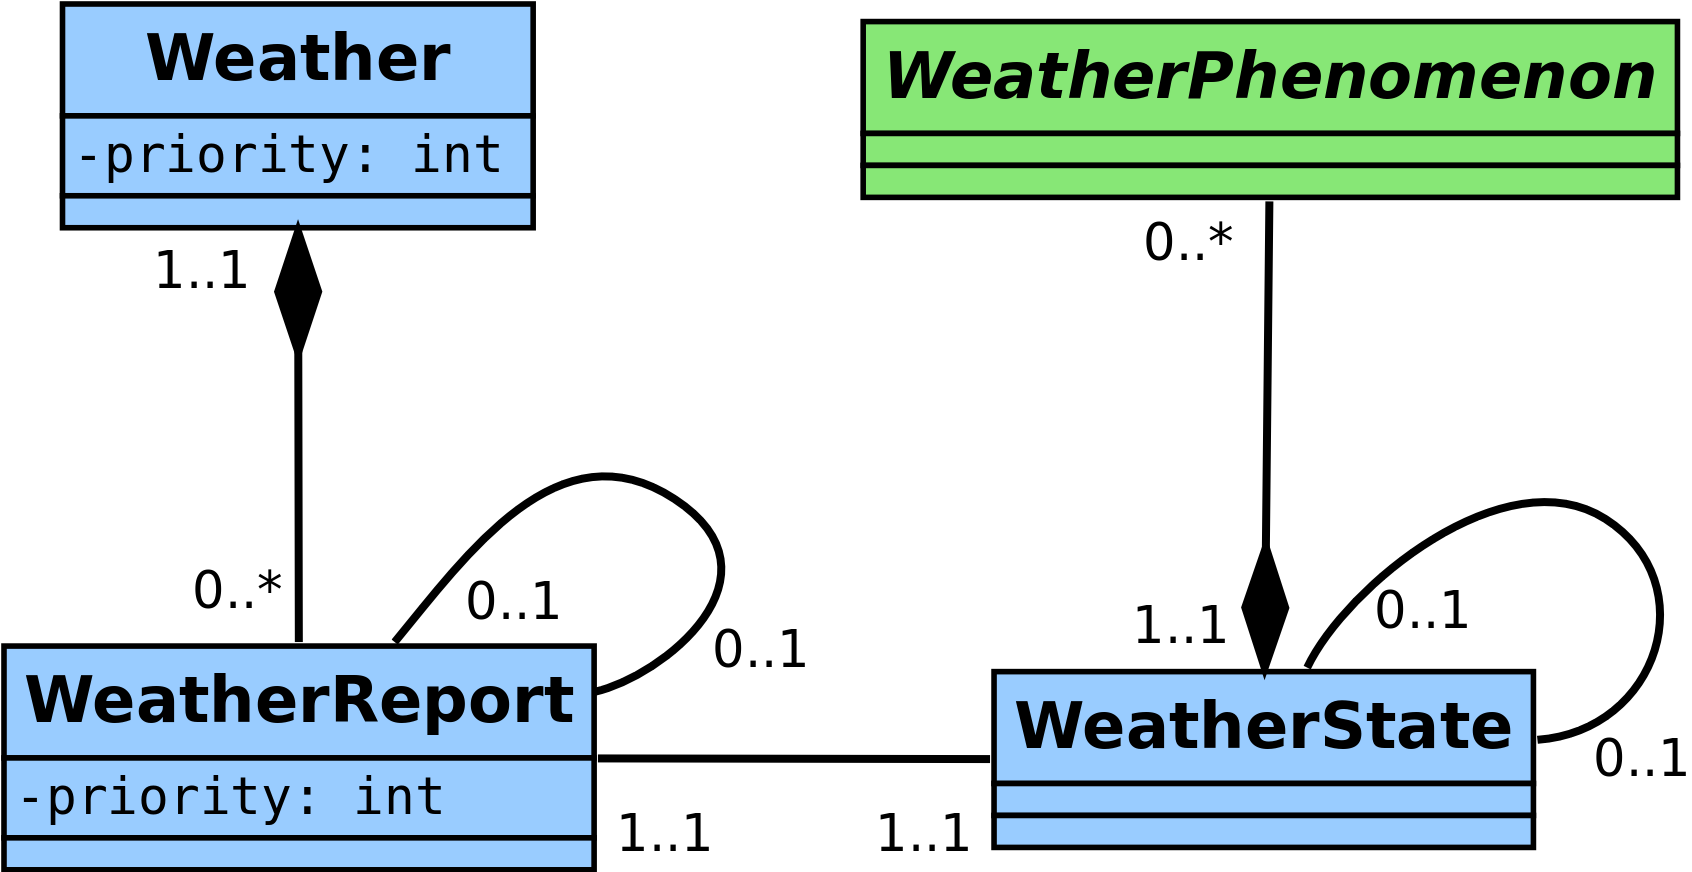
\includegraphics[width=.95\textwidth]{figures/dia/importer-model-simple}
	\end{minipage}

	\vspace{.3em}
	
	\begin{itemize}
	  \item retrieves weather data from local sensors and Internet services.
	  \item generates individuals based on weather data.
	  \item \mbox{provides unit tests for \emph{SmartHomeWeather}.}
	\end{itemize}
      \end{block}

      \begin{block}{Future work}
	Further use cases of \emph{SmartHomeWeather} may be identified. Interoperation with other systems and data sources can be examined:
          \begin{itemize}
            \item Minimising costs for electrical power based on weather data and varying costs for electrical power over time.
	    \item Improving decision making based on both weather data and the buildings' inhabitants' actions.
	    \item Learning from weather situations and their influence on the dwelling.
	    \item Mutual benefits of \emph{Smart Cities} and smart homes utilising \emph{SmartHomeWeather}.
	  \end{itemize}

	  \vspace{4.2mm}
      \end{block}

%      \begin{block}{References}
%        \footnotesize
%	\bibliographystyle{thesis}
%	\bibliography{references}
%      \end{block}
    \end{column}
    % ---------------------------------------------------------%
    % end the column
  \end{columns}

%  \begin{tikzpicture}[remember picture,overlay]
%    \node[inner sep=0pt,xshift=-30cm,yshift=23cm] at (current page.east) {%
%      \begin{postit}%
%        Post-It time!%
%      \end{postit}%
%    }; 
%  \end{tikzpicture}
  
\end{frame}

\end{document}


%%% Local Variables:
%%% TeX-PDF-mode: t
%%% TeX-debug-bad-boxes: t
%%% TeX-master: t
%%% TeX-parse-self: t
%%% TeX-auto-save: t
%%% reftex-plug-into-AUCTeX: t
%%% End:
